
\documentclass[11pt,a4paper]{article}
\usepackage[a4paper,top=2.1cm,bottom=2.2cm,left=2.7cm,right=2.2cm]{geometry}
\usepackage{fontspec}
\setmainfont{DejaVu Serif}
\newfontfamily\armenianfont{DejaVu Serif}
\usepackage{unicode-math}
\setmathfont{DejaVu Math TeX Gyre}
\usepackage{graphicx}
\usepackage{amsmath}
\usepackage{setspace}
\usepackage{indentfirst}
\usepackage{enumitem}
\usepackage{float}
\usepackage{hyperref}
\hypersetup{colorlinks=false,unicode=true,pdfauthor={Մերի Բաղդասարյան},pdftitle={Դիպլոմային աշխատանք}}
\setlength{\parindent}{1.2em}
\setlength{\parskip}{0.38em}
\setstretch{1.18}
\setcounter{tocdepth}{2}
\renewcommand{\contentsname}{ԲՈՎԱՆԴԱԿՈՒԹՅՈՒՆ}
\newcommand{\srcpage}[1]{\par\vspace{0.25em}\noindent\hfill{\scriptsize\color{gray}PDF-ի սկզբնական էջ՝ #1}\par}
\usepackage{xcolor}
\begin{document}
\begin{titlepage}
\begin{center}
{\bfseries ՀԱՅԱՍՏԱՆԻ ԱԶԳԱՅԻՆ ՊՈԼԻՏԵԽՆԻԿԱԿԱՆ ՀԱՄԱԼՍԱՐԱՆ}\\[0.3em]
(ՀԻՄՆԱԴՐԱՄ)\\[1.1cm]
\rule{\textwidth}{0.4pt}\\[0.65cm]
Կիրառական Մաթեմատիկայի և Ֆիզիկայի ֆակուլտետ\\[0.3cm]
Մասնագիտական մաթեմատիկական կրթության ամբիոն\\[0.3cm]
Ինֆորմատիկա (համակարգչային գիտություն) մասնագիտություն\\[2.1cm]
{\LARGE\bfseries ԴԻՊԼՈՄԱՅԻՆ ԱՇԽԱՏԱՆՔ}\\[1.6cm]
ՄԹ 340 ակադեմիական խումբ\\[0.45cm]
Բաղդասարյան Մերի Արտակի\\[1cm]
\textbf{Աշխատանքի թեման}\\[0.4cm]
Մուր--Պենրոուզի պսեվդո-հակադարծ մատրիցի կառուցման\\
ծրագրային գործիքի մշակում և կիրառում\\[1.4cm]
\end{center}
\noindent Աշխատանքի ղեկավար՝ Ա․ Բաբայան\\[0.55cm]
ԿՄՖ դեկանի պ/կ՝ Տ. Մ. Խուդոյան
\vfill
\end{titlepage}
\tableofcontents
\clearpage




\section*{Խնդրի դրվածքը}\addcontentsline{toc}{section}{Խնդրի դրվածքը}

Գծային հանրահաշվի բազմաթիվ կիրառական խնդիրներ հանգում են գծային

հավասարումների համակարգերի Ax=b լուծմանը, որտեղ A∈Rm× n գործակիցների

մատրիցն է, x∈Rn ՝ անհայտների վեկտորը, իսկ b∈Rm ՝ ազատ անդամների




վեկտորը։




Այն դեպքում, երբ (A) մատրիցը քառակուսի է և ոչ սինգուլյար, համակարգն ունի

միակ լուծում, որը կարելի է գտնել հակադարձ մատրիցի միջոցով։ Սակայն

գործնական խնդիրներում հաճախ հանդիպում են ուղղանկյուն կամ սինգուլյար

մատրիցներ, որոնց դեպքում սովորական հակադարձ մատրիցը գոյություն չունի։

Բացի այդ, գծային հավասարումների համակարգը կարող է լինել անհամատեղելի

կամ ունենալ անվերջ թվով լուծումներ։




Նման դեպքերում առաջանում է համակարգի մոտավոր լուծման կամ անվերջ

թվով լուծումներից որոշակի չափանիշով լավագույն լուծման ընտրության

անհրաժեշտությունը։

\section{Գծային հավասարումների համակարգերը և պսևդոհակադարձ մատրիցի անհրաժեշտությունը}

\subsection{Գծային հավասարումների համակարգերի լուծելիությունը}

Դիտարկենք m գծային հավասարումներից և n անհայտներից կազմված

համակարգը՝ Ax=b, A∈Rm× n,x∈Rn,b∈Rm




Հաճախ պատահում է, որ Ax = b հավասարումը լուծում չունի։ Սովորական

պատճառը հավասարումների չափազանց մեծ քանակն է։ A մատրիցն ունի ավելի

շատ տողեր, քան սյուներ, այսինքն՝ հավասարումների քանակը գերազանցում է

անհայտների քանակը (m > n)։ Այդ դեպքում n սյուները կազմում են m-չափանի

տարածության միայն մի փոքր մասը։ Եթե բոլոր չափումները կատարյալ ճշգրիտ

չեն, ապա b-ն գտնվում է A-ի սյունային տարածությունից դուրս։ Բացառման

մեթոդով ստանում ենք անհնարին հավասարում և կանգ ենք առնում։ Սակայն

միայն այն պատճառով, որ չափումներն աղմուկ են պարունակում, մենք չենք կարող

կանգ առնել։




Հիմա կարևորագույն հիմնահարց է հասկանալ,թե որ տեսակի մատրիցի դեպքում

տվյալ գծային հավասարումների համակարգը ինչ լուծում է ունենում։




Սկզբում դիտարկենք քառակուսի մատրիցները։




A-ն քառակուսի մատրից է, քանի որ հավասարումների քանակը հավասար է

անհայտների քանակին։ Եթե ունենք n հավասարում՝ n անհայտով, ապա ստանում

ենք nxn չափանի քառակուսի մատրից։




Հակադարձ մատրիցի սահմանումը։Դիցուք A-ն n×n չափանի մատրից է։

Հակադարձ մատրիցը, եթե գոյություն ունի, նույնպես n×n չափանի է և

նշանակվում է A⁻¹։




Եթե b=Ax և A-ն հակադարձելի է, ապա երկու կողմերը ձախից A⁻¹-ով

բազմապատկելուց ստացվում է x=A⁻¹b։ Հիմնական գաղափարն այն է, որ A-ի

գործողությանը հաջորդող A⁻¹-ի գործողությունը վերադարձնում է սկզբնական




վեկտորը։

A⁻¹A = AA⁻¹ = I; Ax=b ⇒ x=A⁻¹b.




Պետք է տարբերակել պարզապես քառակուսի լինելը և հակադարձելիությունը։

Որոշ քառակուսի մատրիցներ հակադարձ չունեն։ Եթե կա ոչ զրոյական x, որի

համար Ax=0, ապա A-ն չի կարող հակադարձելի լինել. հակառակ դեպքում

A⁻¹Ax=x հավասարությունը կտար x=0 հակասությունը։[2, §1.6]




Ax = b հավասարման ընդհանուր լուծումը x = xp + xn է, որտեղ xp-ն որևէ մասնավոր

լուծում է, իսկ xn-ը՝ զրոյական ենթատարածության ցանկացած վեկտոր։

b-ն զրոյական չէ։ Ձախ մասում կատարվող տողային գործողությունները պետք է

կիրառվեն նաև աջ մասի նկատմամբ։ Ax = b-ն բերվում է ավելի պարզ Rx = d

համակարգի՝ պահպանելով լուծումները։ Դա կազմակերպելու եղանակներից մեկն

է b-ն A մատրիցին որպես լրացուցիչ սյուն ավելացնելը։ b = (b1, b2, b3) աջ մասով

ստանում ենք ընդլայնված մատրիցը [A b]՝։Երբ A-ի վրա կատարում ենք

սովորական բացառումը՝ հասնելով R-ին, նույն գործողությունները կատարում ենք

նաև b-ի վրա։




Լրիվ սյունային ռանգ (r = n) ունեցող ցանկացած A մատրից ունի հետևյալ

հատկությունները.




1. A-ի բոլոր սյուները հենակետային են։




2. Չկան ազատ փոփոխականներ կամ հատուկ լուծումներ։




3. N(A)-ն պարունակում է միայն x = 0 զրոյական վեկտորը։




4. Եթե Ax =b-ն ունի լուծում (կարող է նաև չունենալ), ապա այդ լուծումը միակն է




Լրիվ սյունային ռանգը՝ r = n, նշանակում է, որ ազատ փոփոխականներ չկան. կա

մեկ լուծում կամ լուծում չկա։[1, §3.3]




Լրիվ տողային ռանգ (r = m) ունեցող ցանկացած A մատրից ունի հետևյալ

հատկությունները.




1. Բոլոր տողերում կան հենակետային տարրեր, և R-ը զրոյական տողեր չունի։




2. Ax =b-նլուծում ունի ցանկացած աջ մասի՝ b-ի համար։




3. Սյունային տարածությունն ամբողջ Rm տարածությունն է։




4. A-ի զրոյական ենթատարածությունում կան n−r = n−m հատուկ լուծումներ։




Լրիվ տողային ռանգը՝ r = m, նշանակում է, որ m = n դեպքում կա մեկ լուծում, իսկ

m < n դեպքում՝ անվերջ թվով լուծումներ:[1, §3.3]

\subsection{Նվազագույն քառակուսիների մեթոդը}

Կրկնենք՝ միշտ չէ, որ կարող ենք e = b −Ax սխալը զրոյի հասցնել։ Երբ e = 0, x-ն Ax

= b-ի ճշգրիտ լուծումն է։ Երբ e-ի երկարությունը հնարավորինս փոքր է,𝑥̂ -ը




նվազագույն քառակուսիների լուծումն է։




Երբ Ax = b-ն լուծում չունի, բազմապատկեք AT -ով և լուծենք



\begin{center}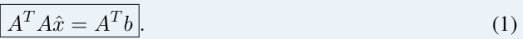
\includegraphics[width=0.579\linewidth]{assets/p05_eq001.png}\end{center}


Նվազագույն քառակուսիների մեթոդի կարևոր կիրառություններից մեկը m

կետերին ուղիղ համապատասխանեցնելն է։ Սկսենք երեք կետից. գտնել (0, 6), (1, 0)

և (2, 0) կետերին ամենամոտ ուղիղը։




b = C + Dt տեսքի ոչ մի ուղիղ չի անցնում այս երեք կետերով։ Պետք է գտնենք երկու

թիվ՝ C և D, որոնք բավարարում են երեք հավասարումների, այսինքն՝ n = 2, m = 3։ t

= 0, 1, 2 պահերին տրված

b = 6, 0, 0 արժեքներին համապատասխանող հավասարումներն են՝






\begin{center}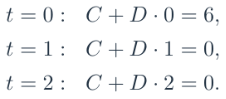
\includegraphics[width=0.251\linewidth]{assets/p06_eq001.png}\end{center}


Այս 3×2 համակարգը լուծում չունի. b = (6, 0, 0)-ն (1, 1, 1) և (0, 1, 2) սյուների գծային

համակցությունը չէ։ Հավասարումներից անմիջապես ստանում ենք A-ն, x-ը և b-ն՝



\begin{center}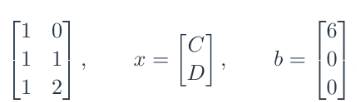
\includegraphics[width=0.395\linewidth]{assets/p06_eq002.png}\end{center}


Ax = b՝ անլուծելի։

Ինչպես e = b − Ax սխալը դարձնել հնարավորինս փոքր։ Լավագույն x-ը (որը

նշանակեցինք 𝑥̂) կարելի է գտնել երկրաչափորեն (e սխալը ուղղահայաց է A-ի

սյունային տարածությանը) և հանրահաշվորեն՝ ATA𝑥̂= ATb հավասարումից։




Երկրաչափական եղանակով։ Յուրաքանչյուր Ax գտնվում է (1, 1, 1) և (0, 1, 2)

սյուներով որոշվող հարթության մեջ։ Այդ հարթության մեջ փնտրում ենք b-ին

ամենամոտ կետը։ Ամենամոտ կետը p պրոյեկցիան է։ A𝑥̂-ի լավագույն




ընտրությունը p-ն է։ Նվազագույն հնարավոր սխալը e = b − p-ն է, որը ուղղահայաց

է սյուներին։ (p1, p2, p3) բարձրություններով երեք կետերը գտնվում են մեկ ուղղի վրա,

քանի որ p-ն պատկանում է A-ի սյունային տարածությանը։ Ուղիղի մոտարկման

ժամանակ 𝑥̂-ը (C, D)-ի լավագույն ընտրությունն է։




Հանրահաշվական եղանակով։ Յուրաքանչյուր b վեկտոր տրոհվում է երկու մասի։

Սյունային տարածության մեջ գտնվող մասը p-ն է, իսկ ուղղահայաց մասը՝ e-ն։ Կա

հավասարում, որը չենք կարող լուծել (Ax = b), և կա հավասարում, որը կարող ենք և

լուծում ենք (A𝑥̂ = p)՝ հեռացնելով e-ն և լուծելով AT A𝑥̂= ATb-ն։



\begin{center}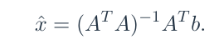
\includegraphics[width=0.234\linewidth]{assets/p06_eq003.png}\end{center}


A𝑥̂= p համակարգի լուծումը թողնում է հնարավոր ամենափոքր սխալը՝ e-ն։




Ցանկացած x-ի համար երկարության քառակուսին՝



\begin{center}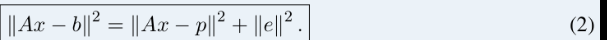
\includegraphics[width=0.672\linewidth]{assets/p06_eq004.png}\end{center}


Սա ուղղանկյուն եռանկյան համար c2 = a2 + b2 Պյութագորասի թեորեմն է։ Ax −p

վեկտորը գտնվում է սյունային տարածության մեջ և ուղղահայաց է ձախ զրոյական

ենթատարածության e վեկտորին։ Ընտրելով x = 𝑥̂ ` Ax−p-ն զրոյի ենք հասցնում։




Մնում է e = (e1, e2, e3) նվազագույն հնարավոր սխալը, որը չենք կարող

փոքրացնել։




Նվազագույն քառակուսիների 𝑥̂ լուծումը հնարավորինս փոքր է դարձնում

E = ∥Ax −b∥2




∥Ax −b∥2-ի մասնակի ածանցյալները զրոյանում են, երբ



\begin{center}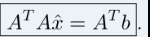
\includegraphics[width=0.166\linewidth]{assets/p07_eq001.png}\end{center}


Նվազագույն քառակուսիների մեթոդի ընդհանուր պատկերը



\begin{center}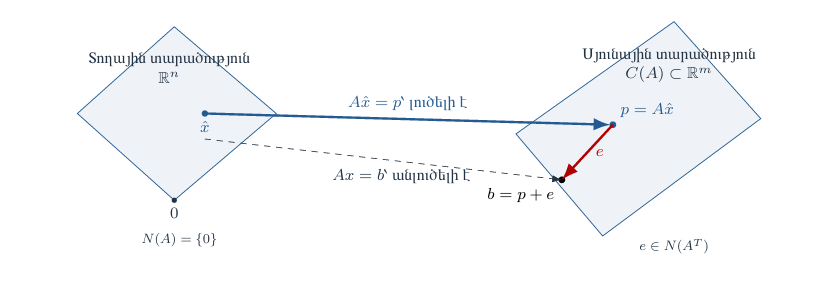
\includegraphics[width=0.951\linewidth]{assets/p07_eq002.png}\end{center}


(p = A𝑥̂ պրոյեկցիան ամենամոտն է b-ին, ուստի 𝑥̂-ը նվազեցնում է E = ∥b−Ax∥2-ը։)




Պատկերված է նվազագույն քառակուսիների մեթոդի ընդհանուր պատկերը։ Ax = b-

ի փոխարեն լուծում ենք A𝑥̂ = p։ e = b −p սխալն անխուսափելի է։




Նկատենք, որ N(A) զրոյական ենթատարածությունը շատ փոքր է՝ ընդամենը մեկ

կետ։ Գծորեն անկախ սյուների դեպքում Ax = 0-ի միակ լուծումն է x = 0-ն։ Ուստի

ATA-ն հակադարձելի է։ AT A𝑥̂= AT b հավասարումը լիովին որոշում է լավագույն 𝑥̂




վեկտորը։ Սխալի համար AT e = 0։

A մատրիցի գծորեն կախյալ սյուները. ինչպիսի՞ն է 𝑥̂-ը




Այս գլխի սկզբից ենթադրել ենք, որ A մատրիցի սյուները գծորեն անկախ են։ Այդ

դեպքում AT A-ն հակադարձելի է, իսկ AT A𝑥̂ = AT b-ից ստանում ենք Ax = b-ի

նվազագույն քառակուսիների լուծումը։Ո՞ր 𝑥̂-ն է լավագույնը, եթե A-ն ունի գծորեն




կախյալ սյուներ։ Դիտարկենք կոնկրետ օրինակ






\begin{center}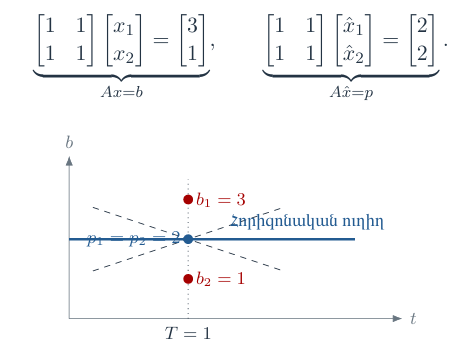
\includegraphics[width=0.787\linewidth]{assets/p08_eq001.png}\end{center}


b1 = 3 և b2 = 1 չափումները կատարվել են միևնույն T պահին։ C + Dt ուղիղը չի կարող

անցնել երկու կետերով միաժամանակ։ Ճիշտ կլինի b = (3, 1)-ը պրոյեկտել A-ի

սյունային տարածության վրա՝ ստանալով p = (2, 2)։ Դա Ax = b հավասարումը

փոխարինում է A𝑥̂= p հավասարմամբ։ Լուծում չունեցող հավասարումը վերածվեց




անվերջ թվով լուծումներ ունեցող հավասարման։ Խնդիրն այն է, որ A-ն ունի գծորեն

կախյալ սյուներ, և (1, −1)-ը պատկանում է նրա զրոյական ենթատարածությանը։

Ո՞ր 𝑥̂ լուծումը պետք է ընտրենք։ Նկարի բոլոր կետագծային ուղիղները T պահին




ունեն նույն երկու սխալները՝ 1 և −1։ Այդ սխալները՝ (1, −1) = e = b−p, հնարավորինս

փոքր են։ Բայց դա դեռ չի ասում, թե կետագծային ուղիղներից որն է լավագույնը։ [1,

§4.3]




\section{Մուր–Պենրոուզի պսևդոհակադարձ մատրիցի տեսական հիմունքները}

\subsection{Պսևդոհակադարձ մատրիցի սահմանումները և դրանց համարժեքությունը}

Դիտարկենք 𝐴̂ : Cn→ Cm գծային արտապատկերումը՝ 𝐴̂x = Ax։ Որպեսզի այն




դառնա փոխմիարժեք, պետք է նրա որոշման տիրույթը սահմանափակել N(A)-ի

լրացուցիչ ենթատարածությամբ։ Բնական ընտրությունն է N(A) ⊥ = R(A*): Այս




դիտարկումը բերում է հետևյալ սահմանմանը։




Սահմանում 1(ընդհանրացված հակադարձի ֆունկցիոնալ սահմանում)։

Դիցուք A ∈ Cmxn Սահմանենք A† : Cm → Cn գծային արտապատկերումը հետևյալ




կերպ՝



\begin{center}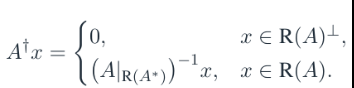
\includegraphics[width=0.392\linewidth]{assets/p09_eq001.png}\end{center}


A†-ի մատրիցն անվանվում է A-ի ընդհանրացված հակադարձ։

Հեշտ է ստուգել, որ AA†x = 0, եթե x ∈ R(A)⊥, և AA†x = x, եթե x ∈ R(A)։ Նմանապես

A†Ax = 0, եթե x ∈ N(A) = R(A∗)⊥, իսկ A†Ax = x, եթե x ∈ R(A∗) = R(A†)։ Ուրեմն AA†-ը




Cm-ի օրթոգոնալ պրոյեկտորն է R(A)-ի վրա, իսկ A†A-ն Cn-ի օրթոգոնալ պրոյեկտորն

է R(A∗)-ի վրա։ Այստեղից առաջանում է Է. Հ. Մուրի առաջարկած երկրորդ




սահմանումը։

Սահմանում 2 (Մուրի սահմանում)։ Եթե A ∈ Cm×n, ապա A-ի ընդհանրացված




հակադարձը միակ A† մատրիցն է, որի համար



\begin{center}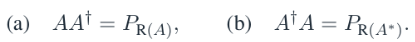
\includegraphics[width=0.460\linewidth]{assets/p09_eq002.png}\end{center}


Մուրն այս սահմանումը տվել է 1935 թվականին, որից հետո այն գրեթե մոռացվել է։

Հնարավոր է՝ պատճառը եղել է դրա ոչ այնքան հարմար սկզբնական նշագրումը։

1955 թվականին Փենրոուզը, ըստ երևույթին տեղյակ չլինելով Մուրի աշխատանքից,

տվել է սահմանման հանրահաշվական տարբերակը։

Սահմանում 3 (Պենրոուզի սահմանում)։ Եթե A ∈ Cm×n, ապա A†-ը միակ n × m




մատրիցն է, որը բավարարում է հետևյալ չորս հավասարումներին՝






\begin{center}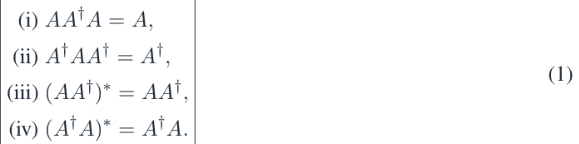
\includegraphics[width=0.640\linewidth]{assets/p10_eq001.png}\end{center}


Առաջին կարևոր փաստը այս երեք սահմանումների համարժեքությունն է։

Թեորեմ 1։ Ընդհանրացված հակադարձի ֆունկցիոնալ, Մուրի և Պենրոուզի

սահմանումները համարժեք են։

Ապացույց։ Արդեն տեսել ենք, որ սահմանում 1-ով կառուցված A†-ը բավարարում է

(a) և (b) հավասարումներին։ Եթե մատրիցը բավարարում է (a) և (b)-ին, ապա

անմիջապես բավարարվում են (iii) և (iv) պայմանները։ Բացի այդ, (a)-ից՝ AA†A =

PR(A)A = A, հետևում է (i)-ը, իսկ (b)-ից՝ նմանապես (ii)-ը։ Քանի որ առաջին

սահմանումը կառուցողական է, գոյության հարցը լուծված է նաև մյուս երկու

սահմանումների համար։ Մնում է ցույց տալ, որ (i)–(iv) պայմանները ենթադրում են

(a), (b), և որ լուծումը միակն է։

Ենթադրենք A†-ը բավարարում է (i)–(iv)-ին։ (ii)-ն ձախից բազմապատկելով A-ով՝

ստանում ենք (AA†)2 = AA†։ (iii)-ի հետ միասին սա նշանակում է, որ AA†-ը

օրթոգոնալ պրոյեկտոր է։ Օգտագործելով (i)-ը և R(BC) ⊆ R(B) հատկությունը՝




ստանում ենք



\begin{center}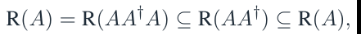
\includegraphics[width=0.400\linewidth]{assets/p10_eq002.png}\end{center}


ուստի R(AA†) = R(A), այսինքն՝ AA† = PR(A)։ Նույն ձևով ապացուցվում է A†A = PR(A∗)




հավասարությունը։

Միակությունն ապացուցելու համար բավական է ցույց տալ, որ (a), (b) կամ (i)–(iv)

պայմանները բավարարող A†-ը բավարարում է առաջին սահմանմանը։ Եթե x ∈

R(A)⊥, ապա (a)-ից AA†x = 0, հետևաբար (ii)-ից A†x = A†AA†x = 0։ Իսկ եթե x ∈ R(A),

ապա գոյություն ունի y ∈ R(A∗), որի համար Ay = x։ Այդ դեպքում A†x = A†Ay = y, քանի

որ A†A-ը պրոյեկտոր է R(A∗)-ի վրա։ Հետևաբար A†x = (A|R(A∗))−1x։

Սա հենց սահմանում 1-ն է։ \textbf{Q.E.D.}




Ընդհանրացված հակադարձը հաճախ կոչվում է Մուր–Պենրոուզի հակադարձ։Եթե

A-ն քառակուսիև հակադարձելի է, ապա A† = A−1, և ընդհանրացված հակադարձն

իսկապես ընդլայնում է սովորական հակադարձ մատրիցի հասկացությունը։




[3, §1]

\subsection{Պսևդոհակադարձ մատրիցի հիմնական հատկությունները[3, §1]}




Նախքան ընդհանրացված հակադարձի ճշմարիտ հատկություններն ապացուցելը,

հարկ է զգուշացնել մի քանի պնդումների մասին, որոնք ընդհանրապես ճշմարիտ

չեն։ Թեև R(A∗) = R(A†), սահմանում 2-ի (b) պահանջը չի կարելի փոխարինել միայն




A†A = PR(A †) գրությամբ՝ առանց A†-ի մյուս պայմանները ապահովելու։

Սովորական հակադարձ մատրիցների համար հաճախ կիրառվում է (AB)−1

= B−1A−1, եթե A-ն և B-ն հակադարձելի են։ Ընդհանրացված հակադարձի համար այս

հատկությունը կարող է խախտվել նույնիսկ այն դեպքում, երբ AB = BA։

Թեորեմ 1։ Եթե A ∈ Cm×n, ապա՝



\begin{center}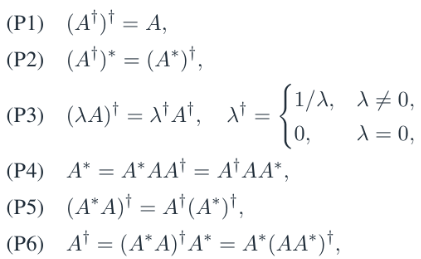
\includegraphics[width=0.466\linewidth]{assets/p11_eq001.png}\end{center}


(P7) (UAV )† = V∗A†U∗, U, V ունիտար։



\begin{center}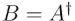
\includegraphics[width=0.083\linewidth]{assets/p11_eq002.png}\end{center}




\begin{center}
\includegraphics[width=0.070\linewidth]{assets/p11_eq003.png}\end{center}


Ապացույց։(P1)Դիտարկենք

մատրիցը և ցույց տանք, որ -ն բավարարում է



\begin{center}
\includegraphics[width=0.070\linewidth]{assets/p11_eq004.png}\end{center}


-ի պսևդոհակադարձին ներկայացվող չորս պայմաններին։ Իրոք,



\begin{center}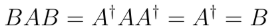
\includegraphics[width=0.300\linewidth]{assets/p11_eq005.png}\end{center}


(ii) պայմանից, իսկ



\begin{center}
\includegraphics[width=0.236\linewidth]{assets/p11_eq006.png}\end{center}


(i) պայմանից։ Բացի այդ,



\begin{center}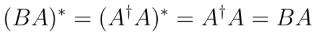
\includegraphics[width=0.350\linewidth]{assets/p11_eq007.png}\end{center}


(iv) պայմանից, և



\begin{center}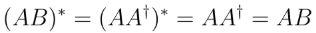
\includegraphics[width=0.350\linewidth]{assets/p11_eq008.png}\end{center}




\begin{center}
\includegraphics[width=0.070\linewidth]{assets/p11_eq009.png}\end{center}




\begin{center}
\includegraphics[width=0.070\linewidth]{assets/p11_eq010.png}\end{center}


(iii) պայմանից։ Ուրեմն

-ն

-ի Մուր–Պենրոուզի պսևդոհակադարձն է։



\begin{center}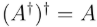
\includegraphics[width=0.108\linewidth]{assets/p11_eq011.png}\end{center}


Միակության շնորհիվ

։



\begin{center}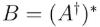
\includegraphics[width=0.111\linewidth]{assets/p11_eq012.png}\end{center}




\begin{center}
\includegraphics[width=0.070\linewidth]{assets/p11_eq013.png}\end{center}




\begin{center}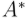
\includegraphics[width=0.070\linewidth]{assets/p11_eq014.png}\end{center}


(P2)

։ Անհրաժեշտ է ստուգել, որ

-ն

-ի պսևդոհակադարձն է։ Համալուծ

տրանսպոնացնելով (i)-ը՝ ստանում ենք



\begin{center}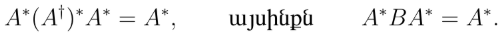
\includegraphics[width=0.556\linewidth]{assets/p11_eq015.png}\end{center}




\begin{center}
\includegraphics[width=0.123\linewidth]{assets/p11_eq016.png}\end{center}


(M2)-ից նույն կերպ՝

։ Բացի այդ՝






\begin{center}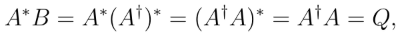
\includegraphics[width=0.441\linewidth]{assets/p12_eq001.png}\end{center}


իսկ



\begin{center}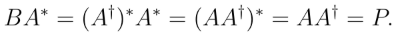
\includegraphics[width=0.438\linewidth]{assets/p12_eq002.png}\end{center}




\begin{center}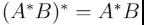
\includegraphics[width=0.159\linewidth]{assets/p12_eq003.png}\end{center}




\begin{center}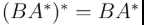
\includegraphics[width=0.159\linewidth]{assets/p12_eq004.png}\end{center}




\begin{center}
\includegraphics[width=0.070\linewidth]{assets/p12_eq005.png}\end{center}




\begin{center}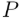
\includegraphics[width=0.070\linewidth]{assets/p12_eq006.png}\end{center}


-ն և

-ն ինքնահամալուծ են, հետևաբար

և

։



\begin{center}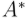
\includegraphics[width=0.070\linewidth]{assets/p12_eq007.png}\end{center}




\begin{center}
\includegraphics[width=0.070\linewidth]{assets/p12_eq008.png}\end{center}


Ստացանք բոլոր չորս պայմանները

-ի և

-ի համար, հետևաբար



\begin{center}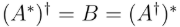
\includegraphics[width=0.199\linewidth]{assets/p12_eq009.png}\end{center}


։



\begin{center}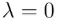
\includegraphics[width=0.070\linewidth]{assets/p12_eq010.png}\end{center}




\begin{center}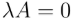
\includegraphics[width=0.080\linewidth]{assets/p12_eq011.png}\end{center}


(P3): Եթե

, ապա

։ Զրոյական մատրիցի պսևդոհակադարձը զրոյական

մատրիցն է, որովհետև այն բավարարում է չորս պայմաններին։ Ուստի

հավասարությունը ճիշտ է։



\begin{center}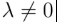
\includegraphics[width=0.070\linewidth]{assets/p12_eq012.png}\end{center}




\begin{center}
\includegraphics[width=0.119\linewidth]{assets/p12_eq013.png}\end{center}




\begin{center}
\includegraphics[width=0.088\linewidth]{assets/p12_eq014.png}\end{center}


Թող այժմ

։ Դնենք

և

։ Ունենք



\begin{center}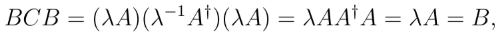
\includegraphics[width=0.553\linewidth]{assets/p12_eq015.png}\end{center}




\begin{center}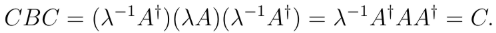
\includegraphics[width=0.549\linewidth]{assets/p12_eq016.png}\end{center}




\begin{center}
\includegraphics[width=0.171\linewidth]{assets/p12_eq017.png}\end{center}




\begin{center}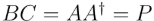
\includegraphics[width=0.171\linewidth]{assets/p12_eq018.png}\end{center}


Միաժամանակ

և

, որոնք ինքնահամալուծ են։



\begin{center}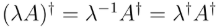
\includegraphics[width=0.242\linewidth]{assets/p12_eq019.png}\end{center}




\begin{center}
\includegraphics[width=0.083\linewidth]{assets/p12_eq020.png}\end{center}


Հետևաբար

, այսինքն՝



\begin{center}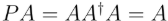
\includegraphics[width=0.186\linewidth]{assets/p12_eq021.png}\end{center}


(P4): (i)-ից ստանում ենք

։ Վերցնելով համալուծ տրանսպոնացումը



\begin{center}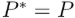
\includegraphics[width=0.083\linewidth]{assets/p12_eq022.png}\end{center}


և օգտագործելով

՝ ունենք



\begin{center}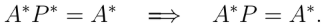
\includegraphics[width=0.358\linewidth]{assets/p12_eq023.png}\end{center}




\begin{center}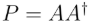
\includegraphics[width=0.100\linewidth]{assets/p12_eq024.png}\end{center}


Քանի որ

, հետևում է առաջին հավասարությունը՝



\begin{center}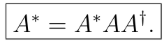
\includegraphics[width=0.184\linewidth]{assets/p12_eq025.png}\end{center}


Երկրորդի համար համալուծ տրանսպոնացնենք (i)-ը՝



\begin{center}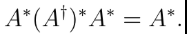
\includegraphics[width=0.207\linewidth]{assets/p12_eq026.png}\end{center}




\begin{center}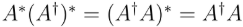
\includegraphics[width=0.269\linewidth]{assets/p12_eq027.png}\end{center}


Իսկ (iv)-ից՝

։ Տեղադրելով՝ ստանում ենք



\begin{center}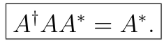
\includegraphics[width=0.184\linewidth]{assets/p12_eq028.png}\end{center}




\begin{center}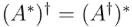
\includegraphics[width=0.146\linewidth]{assets/p12_eq029.png}\end{center}


(P5): Ըստ (P2)-ի՝

։ Հետևաբար բավարար է ապացուցել, որ



\begin{center}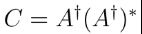
\includegraphics[width=0.158\linewidth]{assets/p12_eq030.png}\end{center}




\begin{center}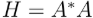
\includegraphics[width=0.103\linewidth]{assets/p12_eq031.png}\end{center}


մատրիցը

մատրիցի Մուր–Պենրոուզի պսևդոհակադարձն է։ Հիշենք



\begin{center}
\includegraphics[width=0.100\linewidth]{assets/p12_eq032.png}\end{center}




\begin{center}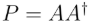
\includegraphics[width=0.100\linewidth]{assets/p12_eq033.png}\end{center}




\begin{center}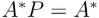
\includegraphics[width=0.110\linewidth]{assets/p12_eq034.png}\end{center}


,

։ Հատկություն (P4)-ից

։ Ուստի






\begin{center}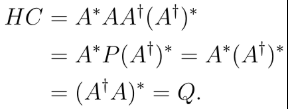
\includegraphics[width=0.319\linewidth]{assets/p13_eq001.png}\end{center}




\begin{center}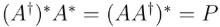
\includegraphics[width=0.244\linewidth]{assets/p13_eq002.png}\end{center}


Մյուս կողմից, (iii)-ից

, ուստի



\begin{center}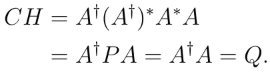
\includegraphics[width=0.299\linewidth]{assets/p13_eq003.png}\end{center}




\begin{center}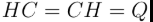
\includegraphics[width=0.169\linewidth]{assets/p13_eq004.png}\end{center}


Այսպիսով

, և երկու արտադրյալներն էլ ինքնահամալուծ են։



\begin{center}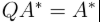
\includegraphics[width=0.111\linewidth]{assets/p13_eq005.png}\end{center}


Հաջորդիվ ստուգենք առաջին երկու պայմանները։ (P4)-ից

, հետևաբար



\begin{center}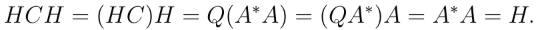
\includegraphics[width=0.594\linewidth]{assets/p13_eq006.png}\end{center}




\begin{center}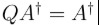
\includegraphics[width=0.110\linewidth]{assets/p13_eq007.png}\end{center}


Իսկ (ii)-ից

, ուստի



\begin{center}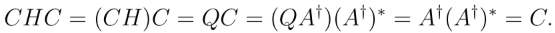
\includegraphics[width=0.614\linewidth]{assets/p13_eq008.png}\end{center}




\begin{center}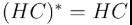
\includegraphics[width=0.146\linewidth]{assets/p13_eq009.png}\end{center}




\begin{center}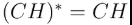
\includegraphics[width=0.146\linewidth]{assets/p13_eq010.png}\end{center}




\begin{center}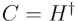
\includegraphics[width=0.086\linewidth]{assets/p13_eq011.png}\end{center}




\begin{center}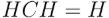
\includegraphics[width=0.121\linewidth]{assets/p13_eq012.png}\end{center}




\begin{center}
\includegraphics[width=0.114\linewidth]{assets/p13_eq013.png}\end{center}


Ստացանք

,

,

և

։ Այսինքն՝

։

Հետևաբար



\begin{center}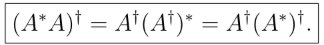
\includegraphics[width=0.358\linewidth]{assets/p13_eq014.png}\end{center}


(P6): (P5)-ի և (P2)-ի համաձայն՝



\begin{center}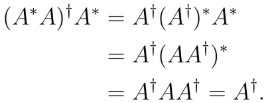
\includegraphics[width=0.297\linewidth]{assets/p13_eq015.png}\end{center}


Այստեղ երկրորդից երրորդ տողում օգտագործեցինք (iii)-ը, իսկ վերջինում՝ (ii)-ը։

Այսպիսով, առաջին նույնությունն ապացուցված է։



\begin{center}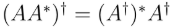
\includegraphics[width=0.191\linewidth]{assets/p13_eq016.png}\end{center}


Երկրորդի համար օգտվենք (P5)-ի վերջում ստացված

հավասարությունից. ունենք



\begin{center}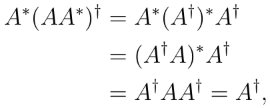
\includegraphics[width=0.299\linewidth]{assets/p13_eq017.png}\end{center}


որտեղ օգտագործվել են (iv)-ը և (ii)-ը։



\begin{center}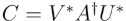
\includegraphics[width=0.139\linewidth]{assets/p13_eq018.png}\end{center}




\begin{center}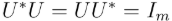
\includegraphics[width=0.191\linewidth]{assets/p13_eq019.png}\end{center}




\begin{center}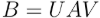
\includegraphics[width=0.111\linewidth]{assets/p13_eq020.png}\end{center}


(P7): Նշանակենք

,

։ Քանի որ

և



\begin{center}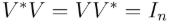
\includegraphics[width=0.188\linewidth]{assets/p13_eq021.png}\end{center}


, ապա



\begin{center}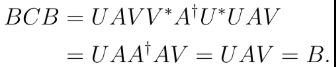
\includegraphics[width=0.372\linewidth]{assets/p13_eq022.png}\end{center}


Նմանապես՝






\begin{center}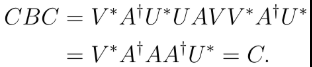
\includegraphics[width=0.345\linewidth]{assets/p14_eq001.png}\end{center}


Մնաց ինքնահամալուծության պայմանները։ Ունենք



\begin{center}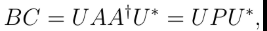
\includegraphics[width=0.295\linewidth]{assets/p14_eq002.png}\end{center}


իսկ



\begin{center}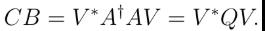
\includegraphics[width=0.294\linewidth]{assets/p14_eq003.png}\end{center}




\begin{center}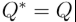
\includegraphics[width=0.085\linewidth]{assets/p14_eq004.png}\end{center}




\begin{center}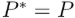
\includegraphics[width=0.083\linewidth]{assets/p14_eq005.png}\end{center}


Քանի որ

և

, ապա



\begin{center}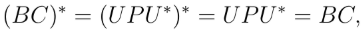
\includegraphics[width=0.403\linewidth]{assets/p14_eq006.png}\end{center}




\begin{center}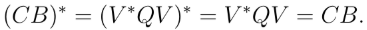
\includegraphics[width=0.407\linewidth]{assets/p14_eq007.png}\end{center}




\begin{center}
\includegraphics[width=0.070\linewidth]{assets/p14_eq008.png}\end{center}




\begin{center}
\includegraphics[width=0.070\linewidth]{assets/p14_eq009.png}\end{center}


Հետևաբար

-ն բավարարում է

-ի նկատմամբ բոլոր չորս պայմանները։

:\textbf{Q.E.D.}



\begin{center}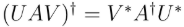
\includegraphics[width=0.204\linewidth]{assets/p14_eq010.png}\end{center}




\begin{center}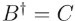
\includegraphics[width=0.083\linewidth]{assets/p14_eq011.png}\end{center}


Միակությունից

, այսինքն՝

Թեորեմ 2։ Եթե A ∈ Cm×n, ապա՝



\begin{center}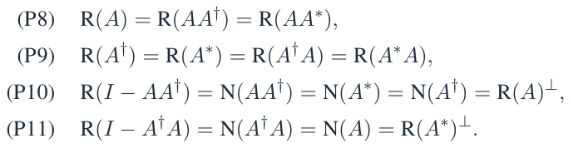
\includegraphics[width=0.632\linewidth]{assets/p14_eq012.png}\end{center}


Պնդում 1։ Եթե A ∈ Cm×n և r = rank(A), ապա գոյություն ունեն B ∈ Cm×r և C ∈ Cr×n




մատրիցներ, որոնց համար



\begin{center}
\includegraphics[width=0.516\linewidth]{assets/p14_eq013.png}\end{center}


Թեորեմ։ Եթե A = BC, որտեղ B ∈ Cm×r, C ∈ Cr×n և r = rank(A) = rank(B) = rank(C), ապա



\begin{center}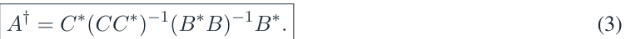
\includegraphics[width=0.695\linewidth]{assets/p14_eq014.png}\end{center}


Ապացույց։ B∗B և CC∗ մատրիցները r×r կարգի, r ռանգով մատրիցներ են, հետևաբար

հակադարձելի են։ Դնենք X = C∗(CC∗)−1(B∗B)−1B∗ և ստուգենք Պենրոուզի




հավասարումները։ Նախ՝



\begin{center}
\includegraphics[width=0.549\linewidth]{assets/p14_eq015.png}\end{center}


հետևաբար (AX)∗ = AX։ Նմանապես



\begin{center}
\includegraphics[width=0.453\linewidth]{assets/p14_eq016.png}\end{center}


ուրեմն (XA)∗ = XA։ Բացի այդ,






\begin{center}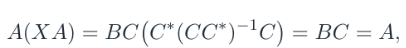
\includegraphics[width=0.450\linewidth]{assets/p15_eq001.png}\end{center}


և (XA)X = C∗(CC∗)−1CC∗(CC∗)−1(B∗B)−1B∗ = X.

Այսպիսով, X-ը բավարարում է չորս պայմաններին, հետևաբար X = A†։\textbf{Q.E.D.}

\subsection{Պսևդոհակադարձի կառուցումը սինգուլյար արժեքների վերլուծության միջոցով (SVD)}

Պսևդոհակադարձ մատրիցը՝ A+

Ճիշտ ընտրված հիմքերի դեպքում A մատրիցը տողային տարածության vi վեկտորը

բազմապատկում է և ստանում սյունային տարածության σiui վեկտորը։ A−1-ը պետք

է կատարի հակառակ գործողությունը։ Եթե Av = σu, ապա A−1u = v/σ։ A−1-ի

սինգուլյար արժեքները 1/σ-ներն են, ինչպես A−1-ի սեփական արժեքներն են 1/λ-

ները։ Հիմքերը փոխվում են տեղերով։ u-երը գտնվում են A−1-ի տողային

տարածության մեջ, իսկ v-երը՝ նրա սյունային տարածության մեջ։

Գոյություն ունի մատրից, որը ui-ն փոխակերպում է vi/σi վեկտորի։ Դա

A+պսևդոհակադարձ մատրիցն է։




A-ի պսևդոհակադարձ մատրիցը

\[A^+=V\Sigma^+U^T.\]



\begin{center}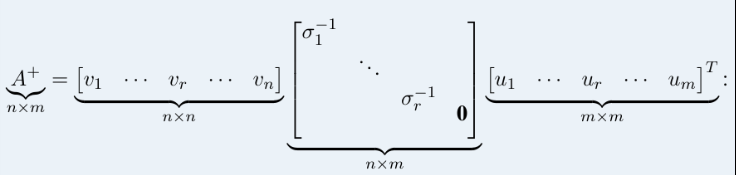
\includegraphics[width=0.815\linewidth]{assets/p15_eq002.png}\end{center}


A+ պսևդոհակադարձը n × m չափի մատրից է։ Եթե A−1-ը գոյություն ունի, ապա A+-ը

համընկնում է A−1-ի հետ։ Այդ դեպքում m = n = r, և UΣV T մատրիցի հակադարձը V

Σ−1U T -ն է։

Նոր՝ A+ նշանակումն անհրաժեշտ է, երբ r < m կամ r < n։ Այդ դեպքում A-ն չունի

երկկողմանի

հակադարձ

մատրից,

սակայն

ունի

նույն

r

ռանգով

A+

պսևդոհակադարձ մատրից՝



\[\boxed{A^+u_i=\begin{cases}\frac{1}{\sigma_i}v_i,&i\le r,\\0,&i>r.\end{cases}}\]


A-ի սյունային տարածության u1, . . . , ur վեկտորները վերադառնում են տողային

տարածության v1, . . . , vr վեկտորներին։ Մնացած ur+1, . . . , um վեկտորները




պատկանում

են

ձախ

զրոյական

ենթատարածությանը,

և

A+-ը

դրանք

փոխակերպում է զրոյի։ Եթե գիտենք, թե A+-ն ինչպես է գործում բոլոր այդ հիմքային

վեկտորների վրա, ապա մենք ամբողջությամբ գիտենք A+ մատրիցը։

Ուշադրություն դարձնենք անկյունագծային Σ մատրիցի պսևդոհակադարձին։ Σ-ի

յուրաքանչյուր ոչ զրոյական σ փոխարինվում է Σ+-ի σ−1-ով։ Σ+Σ արտադրյալը

հնարավորինս մոտ է միավոր մատրիցին։ Դա պրոյեկցիոն մատրից է՝ մասամբ I,

իսկ մնացած մասում՝ զրո։ Մենք կարող ենք հակադարձել σ-ները, բայց ոչինչ անել

չենք կարող զրոյական տողերի ու սյուների հետ։ Հետևյալ օրինակում σ1 = 2, σ2 = 3՝



\begin{center}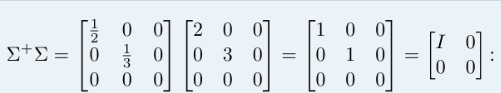
\includegraphics[width=0.554\linewidth]{assets/p16_eq001.png}\end{center}


A+-ը հենց այն n × m մատրիցն է, որի շնորհիվ AA+-ը և A+A-ն դառնում են

պրոյեկցիոն մատրիցներ։



\begin{center}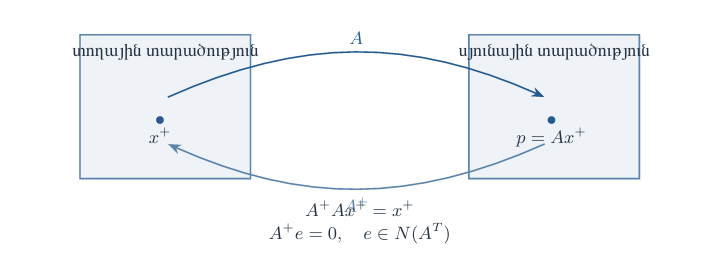
\includegraphics[width=0.990\linewidth]{assets/p16_eq002.png}\end{center}


(յունային տարածության Ax+ վեկտորը A+-ի միջոցով վերադառնում է տողային

տարածության x+ վեկտորին)

Փոխարենը AA−1 = A−1A = I,




AA+ = պրոյեկցիա A-ի սյունային տարածության վրա,

A+A = պրոյեկցիա A-ի տողային տարածության վրա։




Միավորներից կազմված այդ A մատրիցը հանդիպել է նվազագույն քառակուսիների

մեթոդն ուսումնասիրելիս։ Այն չէր բավարարում սյուների գծային անկախության

պահանջին։ Մատրիցն առաջացել էր այն ժամանակ, երբ կատարել էինք երկու

չափում՝ երկուսն էլ t = 1 պահին։ Ամենամոտ ուղիղն անցնում էր 3 և 1 չափված

արժեքների միջնակետով, բայց այդ լավագույն ուղղի թեքությունը որոշելու եղանակ

չկար։




Մատրիցային լեզվով AT A-ն սինգուլյար էր։ AT A= AT b հավասարումն ուներ անվերջ

թվով լուծումներ։ Պսևդոհակադարձը հնարավորություն է տալիս ընտրել

«լավագույն լուծումը»՝ x+ = A+b։

Կրկին գրենք լուծում չունեցող Ax = b հավասարումը և անվերջ թվով լուծումներ

ունեցող AT A = AT b նորմալ հավասարումը՝



\begin{center}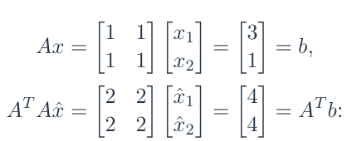
\includegraphics[width=0.387\linewidth]{assets/p17_eq001.png}\end{center}


Յուրաքանչյուր = (1 + c, 1 − c) վեկտոր բավարարում է AT A= AT b նորմալ

հավասարումներին։ Պսևդոհակադարձի նպատակն այդ լուծումներից մեկն

ընտրելն է՝ = x+։



\begin{center}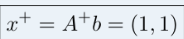
\includegraphics[width=0.204\linewidth]{assets/p17_eq002.png}\end{center}


AT A= AT b և A = p հավասարումների ամենափոքր երկարություն ունեցող լուծումն

է։

Երկրաչափական պատկերացումը հուշում է, թե ինչ պետք է անի A+-ը. A-ի

սյունային տարածությունից պետք է վերադարձնի տողային տարածություն։ Երկու

տարածություններն

էլ

ունեն

r

չափականություն։

Իսկ

ձախ

զրոյական

ենթատարածության e սխալի վեկտորը պետք է վերածվի զրոյի։[1, §7․4]

\section{Պսևդոհակադարձ մատրիցի հաշվարկման ալգորիթմները}

\subsection{Պսևդոհակադարձ մատրիցի կառուցումը լրիվ ռանգով վերլուծության միջոցով[3, §1]}

Սահմանում։ E ∈ Cm×n, rank(E) = r մատրիցը կոչվում է տողային աստիճանաձևի




բերված, եթե



\begin{center}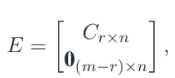
\includegraphics[width=0.194\linewidth]{assets/p17_eq003.png}\end{center}


որտեղ C = (cij)-ի տարրերը բավարարում են՝ (i) cij = 0, երբ i > j; (ii) յուրաքանչյուր

տողի առաջին ոչ զրոյական տարրը 1 է; (iii) եթե cij = 1-ը i-րդ տողի առաջին ոչ




զրոյական տարրն է, ապա C-ի j-րդ սյունը ei միավոր վեկտորն է, որի միակ ոչ

զրոյական տարրը i-րդ դիրքում է։

Օրինակ՝



\begin{center}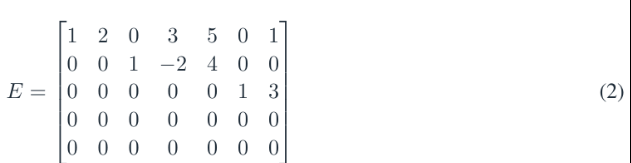
\includegraphics[width=0.645\linewidth]{assets/p18_eq001.png}\end{center}


տողային աստիճանաձև մատրից է։ Ներկայացնենք դրա մի քանի հատկություններ։




Եթե A ∈ Cm×n և rank(A) = r, ապա՝




(E1) Տարրական տողային գործողություններով A-ն միշտ կարելի է բերել EA

աստիճանաձև տեսքի։ Այլ կերպ ասած՝ գոյություն ունի ոչ սինգուլյար P ∈ Cm×m, որի




համար PA = EA։

(E2) Տրված A-ի համար ստացված EA տողային աստիճանաձևը միակն է։

(E3) Եթե EA-ում միավոր սյուները i1, . . . , ir համարներով են, ապա A-ի

համապատասխան սյուները կազմում են R(A)-ի հիմք։ Դրանք կոչվում են A-ի

առանձնացված սյուներ, իսկ մնացածը՝ չառանձնացված սյուներ։ (2)-ի դեպքում

առանձնացված են առաջին, երրորդ և վեցերորդ սյուները։

(E4) Եթե EA-ի ոչ զրոյական տողերից կազմված մատրիցը C-ն է, ապա N(A) = N(EA)

= N(C)։

(E5) Եթե B ∈ Cm×r-ի սյուները A-ի առանձնացված սյուներն են՝ սկզբնական




հերթականությամբ, ապա A = BC։




Ալգորիթմ։ Կամայական A ∈ Cm×n-ի լրիվ ռանգով վերլուծության և ընդհանրացված




հակադարձի ստացում։

(I) A-ն բերել EA տողային աստիճանաձևի։

(II) A-ի առանձնացված սյուներից կազմել B մատրիցը՝ պահպանելով դրանց

կարգը։

(III) EA-ի ոչ զրոյական տողերից կազմել C մատրիցը՝ նույն հերթականությամբ։

(IV) Հաշվել (CC∗)−1 և (B∗B)−1։

(V) Հաշվել A† = C∗(CC∗)−1(B∗B)−1B∗։




Օրինակ։



\[A=\begin{bmatrix}1&2&1&4&1\\2&4&0&6&6\\1&2&0&3&3\\2&4&0&6&6\end{bmatrix}\]


Մատրիցի տողային աստիճանաձևն է



\[E_A=\begin{bmatrix}1&2&0&3&3\\0&0&1&1&-2\\0&0&0&0&0\\0&0&0&0&0\end{bmatrix}\]


Առանձնացված են առաջին և երրորդ սյուները, հետևաբար



\[B=\begin{bmatrix}1&1\\2&0\\1&0\\2&0\end{bmatrix},\quad C=\begin{bmatrix}1&2&0&3&3\\0&0&1&1&-2\end{bmatrix}.\]


Հաշվարկելով՝



\[CC^*=\begin{bmatrix}23&-3\\-3&6\end{bmatrix},\quad B^*B=\begin{bmatrix}10&1\\1&1\end{bmatrix},\quad (CC^*)^{-1}=\frac1{129}\begin{bmatrix}6&3\\3&23\end{bmatrix},\quad (B^*B)^{-1}=\frac19\begin{bmatrix}1&-1\\-1&10\end{bmatrix}.\]


Այսպիսով՝



\[\boxed{A^{\dagger}=C^*(CC^*)^{-1}(B^*B)^{-1}B^*=\frac1{1161}\begin{bmatrix}27&6&3&6\\54&12&6&12\\207&-40&-20&-40\\288&-22&-11&-22\\-333&98&49&98\end{bmatrix}}\]





\clearpage\section*{ՕԳՏԱԳՈՐԾՎԱԾ ԳՐԱԿԱՆՈՒԹՅԱՆ ՑԱՆԿ}\addcontentsline{toc}{section}{ՕԳՏԱԳՈՐԾՎԱԾ ԳՐԱԿԱՆՈՒԹՅԱՆ ՑԱՆԿ}

1. Strang G. Introduction to Linear Algebra. 5th ed. Wellesley-Cambridge Press,

2016.

2. Strang G. Linear Algebra and Its Applications. 4th ed.

3. Campbell S. L., Meyer C. D. Generalized Inverses of Linear Transformations.

4. Horn R. A., Johnson C. R. Matrix Analysis. 2nd ed. Cambridge University Press,

2013.

5. Гантмахер Ф. Р. Теория матриц. 5-е изд., 2010.


\end{document}
